\begin{figure}
    \centering
    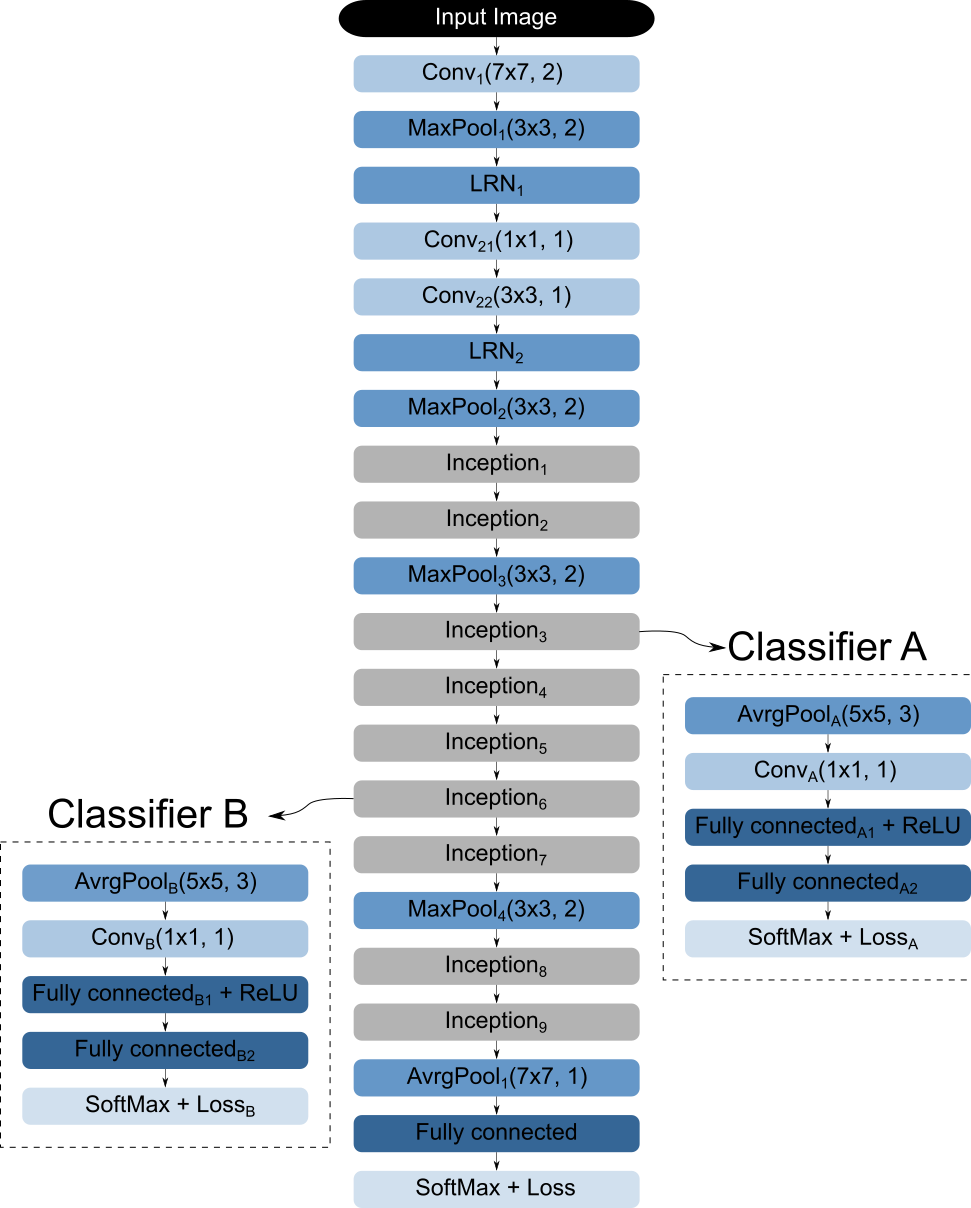
\includegraphics[scale=0.4]{images/figure134.png}
    \caption{GoogLenet network architecture with intermediate classifiers - The GoogLenet network with two classifiers, one in the third inception module and the other in the sixth module. These intermediate classifiers reduce the fading effect of error gradients \cite{img:googlenet}.}
    \label{fig:googlenet2}
\end{figure}

\subsubsection{ResNet}
Residual Neural Network (ResNet) won the ImageNet competition in 2015 with an error rate of 3.6\%. The network developed by a Microsoft research group includes several optimization and regularization techniques from previous models, mainly from GoogLenet. While the characteristic of the GoogLenet network are the inception modules, in ResNet the residual units allowed to train even deeper networks. Among ResNet's main models are nets with 50, 101, 152 layers weights \cite{elgendy2020}, more than double the number of GoogLenet with 22 layers.

Like GoogLenet, the ResNet network can be divided into three parts, the first and last part following the GoogLenet architecture, and the intermediate layers include the residual units. Input layers that allow for a considerable reduction in image size include a convolution layer with 64 channels and 7 x 7 with stride=2 filters, followed by a 3 x 3 MaxPooling layer with stride=2. The last part of the network, the classification structure, has the same layers as GoogLenet, the average Global Pooling layer of dimension 1024 and only a fully connected layer with 1000 units representing the classes. Remembering that the replacement of the flattering process by the global average allowed to reduce the proportion of parameters in the last layers.

\begin{figure}
    \centering
    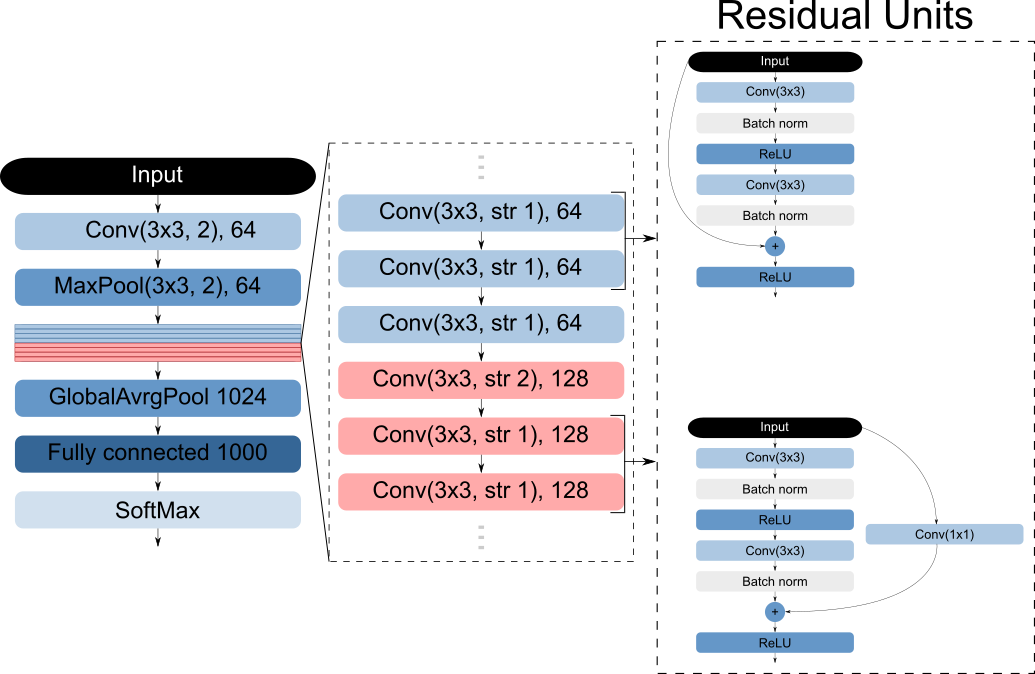
\includegraphics[scale=0.4]{images/figure135.png}
    \caption{ResNet network architecture - The overall structure of the ResNet network can also be divided into three parts. Similar to GoogLenet, it contains a convolutional layer and pooling to reduce image dimensions. A part with residual unit modules, and at the end a global pooling layer and a Full Connect for classification \cite{geron2019}.}
    \label{fig:figure135}
\end{figure}

As described in section GoogleLenet network by adding more layers, the number of parameters can increase in a way that makes training difficult, not only due to the limitations of computational resources, but also due to the possibility of overfitting and delay in the convergence of the algorithm. The GoogLenet model adopted several optimization and regularization approaches, including intermediate classification layers to ensure that the model could converge, avoiding the disappearance of the weights (vanishing gradients), which at times tended to zero \cite{geron2019}.

One of the ResNet techniques that helped to speed up convergence in training was batch normalization. This method became a reference for several CNN models, as until that time each model adopted different approaches to training, such as the intermediate classes of GoogLenet \cite{johnson2019}. Normalization is applied individually by layer, and data normalization occurs based on the statistics of the minibatch clusters adopted in training, which were quickly seen in MLP \cite{zhang2020dive}. In ResNet networks, normalization is applied to the data at the time of transition between the convolution layer and the activation layer.

Even though they managed to converge deeper networks, it was identified in the models that there was a degradation in the accuracy when adding more layers \cite{he2016}. Previously, there was the intuition that when starting from a model with a reduced number of layers to a deeper network, the error should not increase, because at least the deeper network would have part of its layers copied from the other network and the other part would function as identity functions. With more layers, the optimization of a model becomes more complex even for problems easily mapped into smaller networks \cite{he2016}. The idea at ResNet to deal with this complexity was to force the layers to perform the output mapping by including as a reference the input itself, that is, a residual mapping \cite{geron2019}.

In the common mapping of the layers in Figure \ref{fig:figure136}, one imagines that from an training example $\mathbf{x}$, the training seeks to establish an expected response $\mathbf{(x)}$. In the case of residual mapping, a deviation of the input data (x) is included in the output to force a h(x)-x model. This is expected to make it easier to optimize a model with reference, the residual mapping, and that it can quickly adjust to identity functions, ensuring that the layers at least establish the performance of the previous layers \cite{zhang2020dive}. Deviations, residual connections, also minimize the effects of the disappearance of weights, as they allow an alternative flow of gradients, contributing to the back-propagation of the error \cite{elgendy2020}.

\begin{figure}
    \centering
    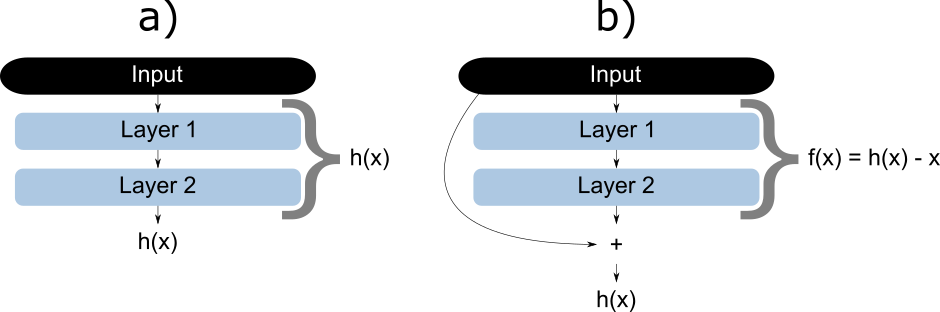
\includegraphics[scale=0.4]{images/figure136.png}
    \caption{Conventional and residual mapping of the ResNet network - a - Traditional mapping of the input and output layers; b - Mapping on a residual unit of the ResNet network. In common mapping, an input x is sought to establish an expected response h(x). The residual model includes an input deviation (x) in the output to force a h(x)-x response \cite{geron2019}}.
    \label{fig:figure136}
\end{figure}

The residual connection starts from the input of a residual unit towards its output, adding the input information with the response before the activation layer ReLu (Figure  \ref{fig:figure137}). Each residual unit has two layers of 3 x 3 convolution, with stride=1 and padding configuration to maintain dimensions. Between the two layers there is a normalization layer preceding a ReLu activation.

\begin{figure}
    \centering
    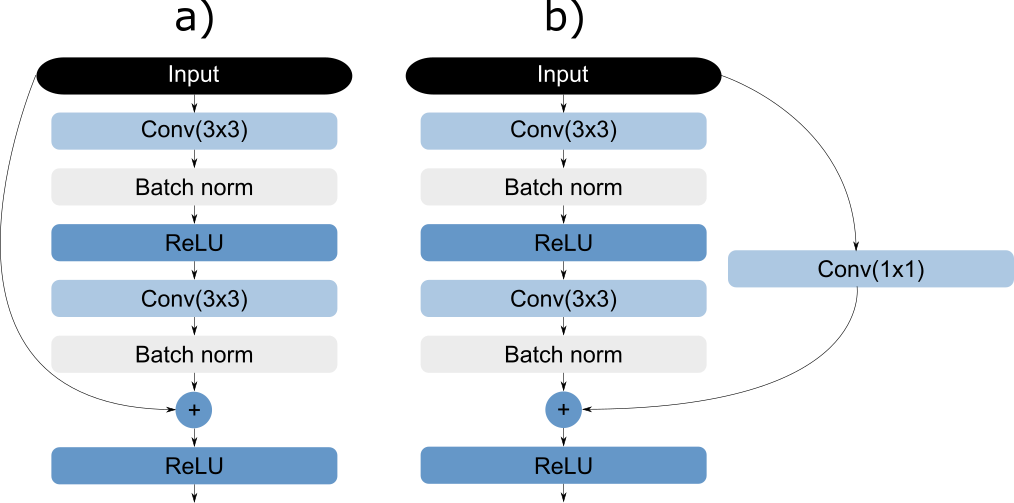
\includegraphics[scale=0.4]{images/figure137.png}
    \caption{Residual unit of the ResNet network - In the middle part of the ResNet network there is a sequence of modules with residual units. Each residual unit has two layers of convolution interspersed by a ReLu activation and a normalization that is also applied to the output of the convolutions \cite{geron2019}}.
    \label{fig:figure137}
\end{figure}

After a sequence of residual units of the same configuration, between the modules, the number of channels is doubled and, at the same time, the width and height of the channels is reduced by half. Between the residual units, no pooling layers are used, thus, to reduce the dimensions of the channels, stride=2 is used in the convolution that encloses a module. In this way, in the last residual unit of the modules, the input has a different dimension than the output. To be able to add the values, it is necessary to correct the dimensions of the input with a 1 x 1 convolution of stride=2 and the same number of channels as the output of the unit    \cite{zhang2020dive}.

The structure of the modules with the residual units resemble the blocks of the VGG network, in which each block presents a sequence of convolution layers with the same dimensions, and always 3 x 3 filter . From one block to another in the VGG, the number of channels also doubles and the height and width are halved, in this case by the MaxPooling effect. ResNet features 4 modules, where the number of residual units varies from model to model as indicated in Figure \ref{fig:figure138}. The ResNet-34, for example, with 34 weight layers contains, respectively, in the four modules, three residual units with 64 channels output, four units with 128 channels, six units with 256 channels and three units with 512 channels \cite{he2016}.

\begin{figure}
    \centering
    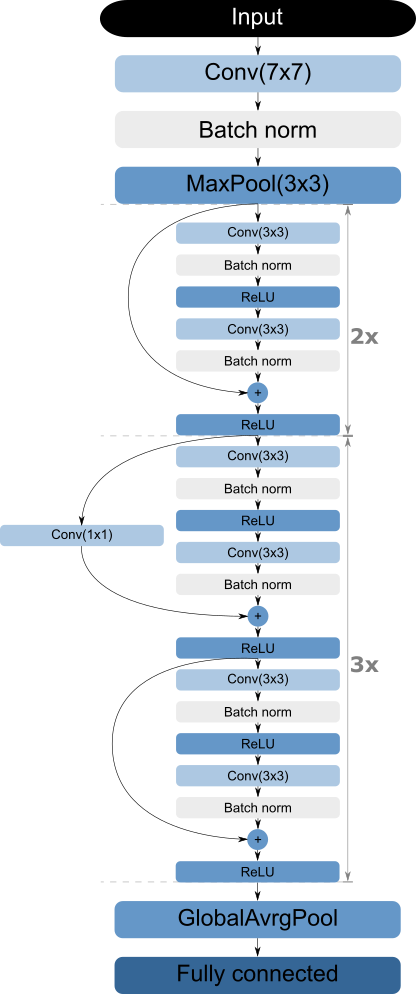
\includegraphics[scale=0.4]{images/figure138.png}
    \caption{ResNet standard architecture - There are several versions of ResNet, with the beginning and the end of the networks being similar, and what usually changes is the amount of residual units in each of the four modules, in the middle part of the network \cite{geron2019}.}
    \label{fig:figure138}
\end{figure}

\section{Transfer learning} \label{transferlearning}
Training a neural network from scratch is a complex task, as it requires an enormous amount of data and computational power \cite{elgendy2020}. In many cases we may not have enough of either, but that doesn't stop us from creating our models. For this we have a technique known as transference learning, which basically consists of using already trained models to solve our problems. In this case we assume that many of the factors that explain the $P_1$ context (situation in which the model was trained) can also explain our new $P_2$ context \cite{goodfellow2016}.

We were able to use this technique because even models trained for different problems end up learning to detect similar characteristics in the earlier layers, with greater specification in the deeper layers. We can see this in Figure \ref{fig:figure139}, where we have the representation of four different networks, the first aimed at working with the image of people, the second with cars, the third with elephants and the last with chairs. Even though these are completely different objects, the networks learn, in the initial layers, to detect edges and corners, which are characteristics shared by all items.

\begin{figure}
    \centering
    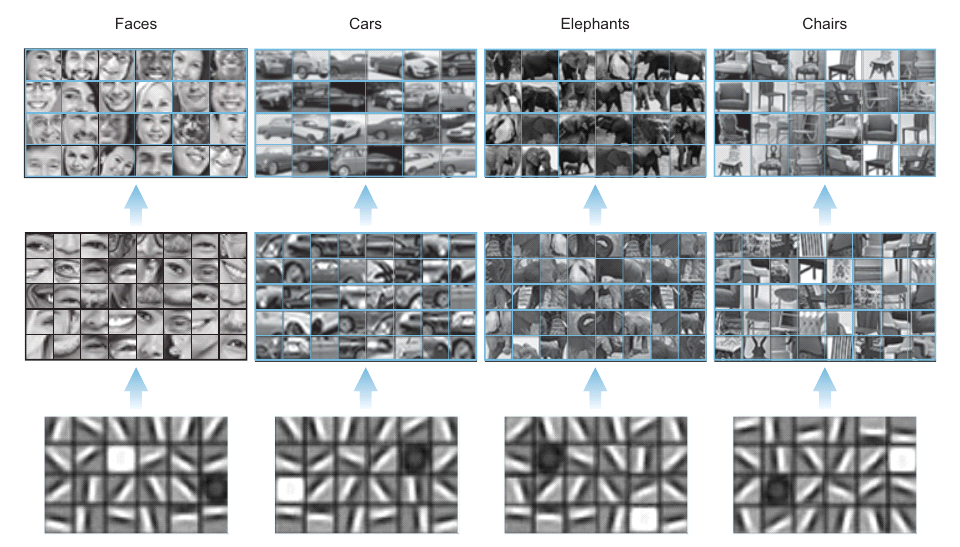
\includegraphics[scale=0.4]{images/figure139.png}
    \caption{Different CNN's and their feature maps in different layers - In the first column we have the features learned by a network specialized in working with human faces, in the second column with cars, in the third with elephants and in the fourth with chairs \cite{elgendy2020}.}
    \label{fig:figure139}
\end{figure}

There are three main ways to carry out the transfer of learning \cite{elgendy2020}, each of which fits better in one scenario or another, they are:

\begin{itemize}
\item Use a pre-trained network as a classifier
\item Use a pre-trained network as a feature extractor
\item Use a pre-trained network for fine tuning
\end{itemize}

The method of using a pre-trained network as a classifier is better when our problem has a domain very similar to the already trained network that we are going to use, as we only have to fit it into our use, not requiring additional training.

The method using a pre-trained network as a feature extractor  is useful when we are solving a problem that has several common features with a pre-trained network but not in a way that we can use as in the previous approach. What we do then is “freeze” the layers of the network that extract features (ie, the layers of convolution) and replace the fully connected network at the end, putting in its place another network that we classify according to our needs, and we train it.

\begin{figure}
    \centering
    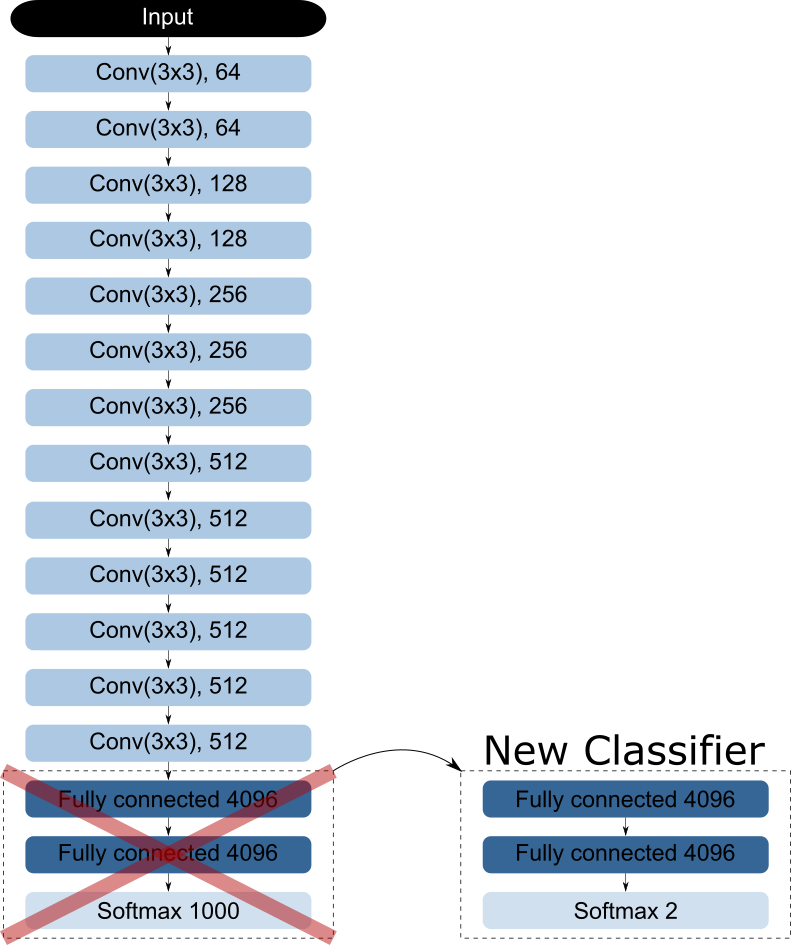
\includegraphics[scale=0.4]{images/figure140.png}
    \caption{VGG-16 Network - We have, from top to bottom, the “frozen” layers, the layers that will be removed and the layer that will be added and trained \cite{elgendy2020}}
    \label{fig:figure140}
\end{figure}

In Figure \ref{fig:figure140}, we have an example from the book by Mohamed Elgendy \cite{elgendy2020}, where he wanted to carry out the classification of dogs and cats. The VGG-16 Network was chosen because it was trained on the ImageNet database, which contains many examples of dogs and cats, so it could adapt well to our problem.

The two previous methods are used when we have a similar domain, since this one, the third method, which uses the pre-trained network for fine tuning, fits into problems that have very different properties. Even in these cases, we were able to use pre-trained networks, for the reasons mentioned above, that networks, especially in their initial layers, learn to detect similar characteristics, becoming more specific according to their depth \cite{elgendy2020}.

In the method that uses the pre-trained network for fine tuning, we have some possibilities. One of them is to “freeze” the first convolutional layers and retrain the rest of the network, what we'll be doing then is fine-tuning (also known as fine-tune) in the deeper layers of the network, so that they can adapt to our current problem. . And the other is not to "freeze" any layer and retrain the entire network, in this case, even having to spend more time and more data is needed, the network tends to converge more quickly to an optimal solution, in comparison to a random initiation \cite{elgendy2020}.

In the book “Deep Learning  for Vision Systems” by Mohamed Elgendy, some tips are presented on how to choose the best learning transfer technique for some types of scenarios, which are presented in Table \ref{table:compareMethods}:

\begin{center}
\begin{table}
    \begin{tabular}{| m{0.14\textwidth} | m{0.14\textwidth} | m{0.30\textwidth} | m{0.25\textwidth} |} \hline
        \textbf{Scenario}& \textbf{Amount of data available}& \textbf{Similarity between the pre-trained network and the new database}& \textbf{Method}\\ \hline
        
        1& Small& Similar& Use a pre-trained network as a classifier\\ \hline
        2& Great& Similar& Fine tune on fully connected network\\ \hline
        3& Small& Very different& Fine-tuning on a part of the network\\ \hline
        4& Great& Very different& Fine tuning across the network\\ \hline
    \end{tabular}
    \caption{Different scenarios where we can use learning transfer (Adapted from \cite{elgendy2020}).}

    \label{table:compareMethods}
\end{table}
\end{center}


\section{Neural networks in practice}
When studying the different models of CNN's we realized that the main factor to improve the accuracy of the networks was the increase in the number of layers, making the networks deeper. It is noteworthy that the construction of deeper models was only possible due to the evolution of hardware performance, especially memory and processing units, and the development of more specific software, known as frameworks for Deep Learning  \cite{zhang2020dive}.

The training of networks involves thousands of operations with multidimensional elements, that is, n-dimensional arrays with arbitrary number of axes, known as tensors \cite{zhang2020dive}. Tensors with only one dimension mathematically correspond to vectors, while tensors with two dimensions are matrices. In the case of CNN's networks, the inputs are often colored images that can be interpreted as three-dimensional tensors: image height, width and volume (RGB channels). Within the network, a series of multiplications and additions takes place from the input tensor, resulting in different three-dimensional tensors.

The performance of all operations is only possible due to the processing units of the machines, which allow the interaction of the arithmetic logic unit (ALU) with the memory. When the first networks were developed, the main processing resource was the CPU's, a general purpose processor where the ALU only performs one calculation at a time. As it has more general applications, it needs constant access to memory for reading instructions and storing data, which is a disadvantage in relation to processing time, known as the “von Neumann bottleneck” (Developers 2021). Generally, to make memory access faster, more sophisticated technologies are integrated into caches, but their size is limited due to cost \cite{zhang2020dive}.

The storage and processing limitations related to a single CPU make it impossible to train deeper networks. What allowed the evolution of networks was the adaptation of processing units with more specific applications. Most modern networks are implemented based on graphics processing units (GPU's). These components were originally developed for graphics applications, mainly for video game rendering \cite{goodfellow2016}. However, much of the GPU's processing approach has also proved to be compatible with the calculations needed to train neural networks.

The GPU achieves greater processing power than a CPU, as it integrates several ALU's in a single processor, which allows thousands of operations to be performed simultaneously (Developers 2021). This strategy is ideal for applications that are suited to parallel processing, such as matrix multiplication in a neural network, which involve independent operations \cite{goodfellow2016}. GPUs were built to perform simpler operations without involving as many branches as is often necessary in CPU workflow. Most network training calculations are predictable, with algorithms that do not require sophisticated controls \cite{goodfellow2016}.

If, on the one hand, network operations do not require great computational complexity, on the other, they demand large amounts of memory. During training you need to store parameters, activation values, and gradients, that is, an amount of data beyond the cache limit associated with the CPU \cite{goodfellow2016}. In this sense, in addition to allowing parallel processing, reducing training time, the GPU also offers a greater amount of memory.

The use of the GPU for training networks became even more common after the adaptation for more general purposes. One of NVIDIA's leading GPU models supports CUDA programming for developing arbitrary code similar to the C language \cite{goodfellow2016}. Thus, the GPU can execute different routines that are not only associated with rendering subroutines.

To ensure high-performance GPU codes, different libraries have been built over the years that deal with numerical computation, mainly involving convolutions and other operations with tensors \cite{goodfellow2016}. Thus, in the development of networks it is not necessary to know the programming at the CUDA level, which is more complex and involves parallel and distributed computing. Generally these libraries, or frameworks, are supported on both GPU and CPU. The first generations of many frameworks were developed through partnerships between Universities and large companies interested in Deep Learning . Some of the more common libraries, highlighted in Table \ref{table:IAframework}, are PyTorch and Caffe2 maintained by Facebook, TensorFlow by Google, MXNet by Amazon, and CNTK by Microsoft \cite{johnson2019}.

\begin{center}
\begin{table}
    \begin{tabular}{| c | c | c |} 
        \hline
        \textbf{Framework}& \textbf{Developer}& \textbf{Predecessor Framework}\\ \hline
        
        Caffe& UC Berkeley& -\\ \hline
        Caffe2& Facebook& Caffe\\ \hline
        Torch& NYU / Facebook& -\\ \hline
        PyTorch& Facebook& Torch\\ \hline
        Theano& U Montreal& -\\ \hline
        TensorFlow& Google& Theano\\ \hline
        PaddlePaddle& Baidu& -\\ \hline
        MXNet& Amazon& -\\ \hline
        Jax& Google& -\\ \hline
        CNTK& Microsoft& -\\ \hline
        Chainer& Community& -\\ \hline

    \end{tabular}
    \caption{Main frameworks for Deep Learning  - To facilitate the manipulation of tensors and the use of GPU's, different frameworks were developed. Most of the first generations of frameworks emerged as partnerships between universities and large companies \cite{johnson2019}.}
    \label{table:IAframework}
\end{table}
\end{center}

Even with the GPU performance increase in relation to the CPU to train the networks, in many cases, a single machine is not enough for all the processing. With the possibility of parallelism, it became common to distribute the workload among several machines. However, building your own GPU network is a high investment, and the technology would also depreciate in a few years as GPU models are rapidly evolving to keep up with growing networks \cite{wangenheim2018}. An alternative for local networks is to use cloud GPU servers offered by providers like Amazon, Google, Microsoft and others.

In recent years, the offer of cloud services to train CNN's has increased, with costs based on the type of GPU technology available, processing time and amount of storage \cite{wangenheim2018}. Some providers offer some free services. The networks can be developed directly on platforms offered by the providers themselves, which generally have an IDE based on Jupyter Notebooks. Each platform has facilities for certain frameworks, usually for those libraries that also provide support \cite{wangenheim2018}. GoogleCloud, for example, features several tools to integrate with TensorFlow.

GoogleCloud offers, in addition to GPU services, the alternative of accessing TPUs as cloud computing resources. The TPU (Tensor Processing Units) is specifically designed to work with neural networks and functions as a specialized matrix processor. As the sequence of calculations is already known, several multipliers and adders were connected, forming a matrix of operators, called systolic matrix (Developers 2021). An advantage of the TPU over CPU and GPU is the reduction of the von Neumann bottleneck, as data is all loaded from memory at once, not requiring access during calculations (Developers 2021).

In the topic about backpropagation an example of an MLP network application for digit recognition that we implemented in the Python language was presented. In the code, the network structure, the training steps and the functions were manually developed, mainly using libraries that deal with calculations in Multidimensional Arrays, such as Numpy. In the MLP example, when manipulating data as numpy's array, no inconsistencies arose and we also didn't face very complex operations, because until that moment the applications didn't involve very dense networks, which required several optimizations and regularizations. In larger network models, using the backpropagation algorithm is a greater challenge and it can often be difficult to ensure convergence just using traditional numerical computation libraries \cite{adrian2017}.

On the other hand, the frameworks we just presented, such as TensorFlow and Pythorch, were built specifically to deal with Deep Learning , and can, for example, automatically provide various optimization and regularization functions. Deep Learning  frameworks generally feature a multidimensional data structure, treated as a tensor class, which replaces the numpy’s “ndarray” \cite{zhang2020dive}. This tensor data structure has some advantages over the traditional numpy array that is better suited to data manipulation in networks. The first point is that numpy defaults to 64 bits precision, whereas tensors generally use 32 bits. Since 32 bitsaccuracy is sufficient to work with networks, reducing data size takes up less memory and makes operations faster \cite{geron2019}.

By default, the manipulation of variables is directed towards calculations in the CPU, however, when different CPU and GPU devices are available, it may be interesting to distribute calculations and storage \cite{zhang2020dive}. Unlike Numpy, Deep Learning  frameworks support handling multiple devices at the same time \cite{zhang2020dive}. Previously we highlighted that the purpose of using GPUs in networks is to speed up training, mainly by adopting distributed and parallel processing, however, if data handling is not adequate, there will be many transfers between devices, thus, processing time may increase \cite{zhang2020dive}. Generally, when using the frameworks configured with the GPU's and CPU's, it is not necessary to worry about how these transfers occur, as the processing is optimized based on computational graphics \cite{geron2019}.

What has made CNN's even more popular even outside academic circles is the development of programming interfaces that make the construction and training of neural networks simpler. Keras, one of the best known APIs for Deep Learning  at a high level, was developed by François Chollet as a research project, which was made available as open source in 2015 \cite{geron2019}. It was written in Python and functions as an underlying computation engine that runs under different backend frameworks, some identified in Figure \ref{fig:figure142}, which support numerical computation, such as TensorFlow, Theano, CNTK, and MxNet \cite{geron2019}.

Much of the work with neural networks can be implemented directly with the high-level API, including the design of the architecture, functions, training algorithm, optimizers and regularization modules. For implementations that need more customization, it is necessary to resort to lower level frameworks, such as TensorFlow, created by a Google research group and released as free software in 2015, has its own keras implementation, tf.keras \cite{geron2019}.

The tf.keras API has only TensorFlow as its backend (Figure \ref{fig:figure142}), but it has greater facilities to integrate with backend customizations. The addition of new codes can be done from the Python language and the API automatically converts to functions of type TensorFlow that are based on C++ \cite{geron2019}. Often these adaptations occur when more control is needed, or to customize functions, layers, regularization modules, initialization processes, or evaluation measures \cite{geron2019}.

Currently the last stable version of TensorFlow is 2.4, the first version of TensorFlow 2.0 being released in March 2019 (Developers 2020). While in versions 1.0, the symbolic module is the central part \cite{geron2019}, mainly due to the preference for the static graphics approach, from versions 2.0 onwards, there was a more imperative programming similar to PyTorch, and that defaults to dynamic graphics \cite{zhang2020dive}. The static module seeks greater code optimization, and after defining the entire process and building the graph, there is no longer any dependence on the code \cite{johnson2019}. In dynamic format, the construction and execution of graphics cannot be unlinked, as they occur simultaneously. Generally, dynamic graphics are easier to debug and have fewer inconsistencies.

\begin{figure}
    \centering
    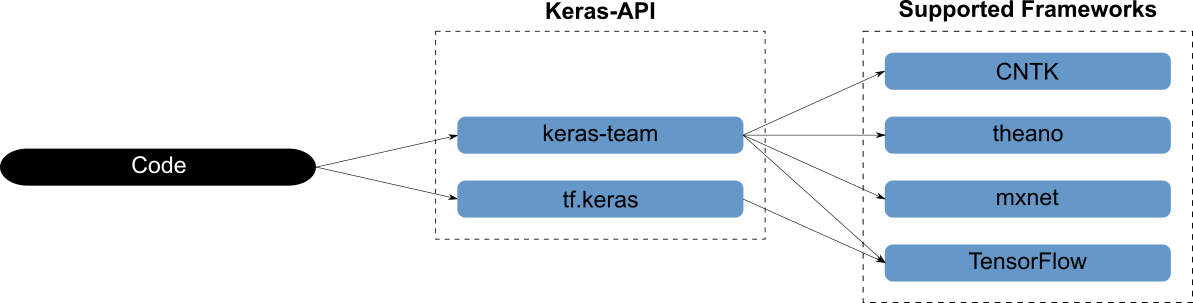
\includegraphics[scale=0.37]{images/figure142.png}
    \caption{ResNet standard architecture - There are several versions of ResNet, with the beginning and the end of the networks being similar, and what usually changes is the amount of residual units in each of the four modules, in the middle part of the network \cite{geron2019}.}
    \label{fig:figure142}
\end{figure}







